We assess our method by determining how the different offloading strategies satisfy user-specified deadlines in a multi-cluster environment.

\subsection{Experimental Setup}\label{subsec:experimental-setup}

\begin{figure}[h]
    \centering
    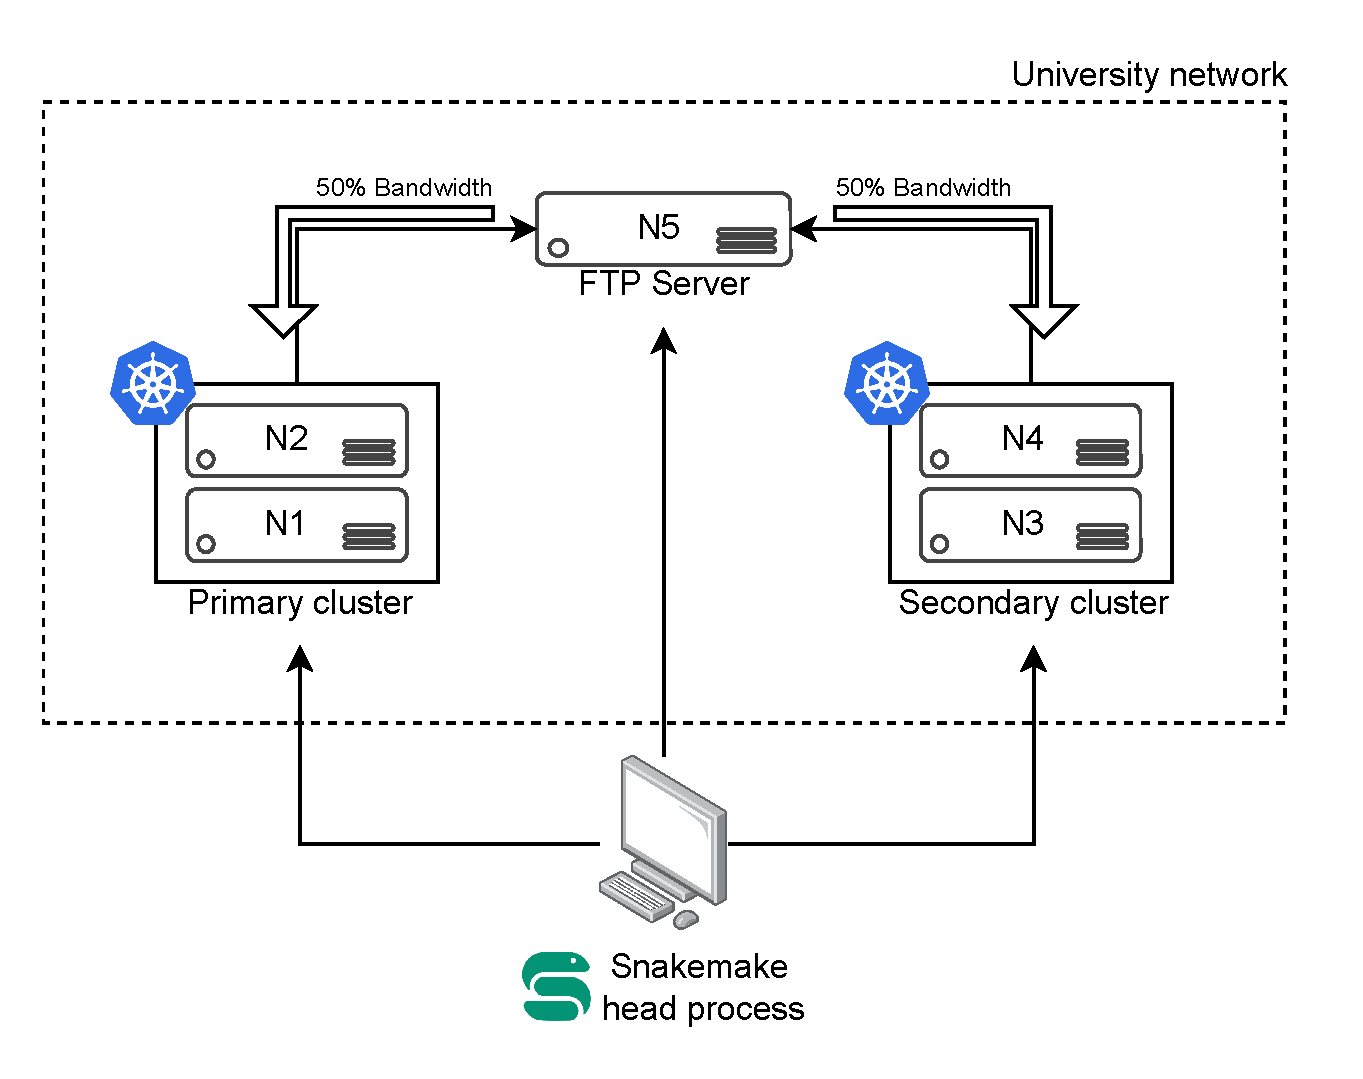
\includegraphics[width=1\linewidth]{./img/evaluation/experimental_setup.drawio.pdf}
    \caption{Kubernetes cluster setup for the experiments}
    \label{fig:experimental_setup}
\end{figure}

The following sections provide a description of the infrastructure configuration used for the evaluation, a brief account of the implementation of our approach, and an overview of the workflows used to assess our strategies.
\subsubsection{Infrastructure}
Fig.~\ref{fig:experimental_setup} shows the setup used for all experiments in this paper.
We employ two Kubernetes-based computing environments, referred to as the primary and secondary clusters. A Snakemake head process (version 9.5.1) runs on a local workstation with macOS 15.5 and connects, via a virtual private network (VPN), to two Kubernetes clusters that reside within the same university subnet. We use the tc utility\footnote{\url{https://linux.die.net/man/8/tc}} to allocate 50\% of the available bandwidth to the IP addresses of each Kubernetes cluster.
This is to keep FTP data transfer rates approximately constant between non-offloading and offloading scenarios.
Otherwise, when both clusters are in use and potentially twice as many jobs run concurrently, the available bandwidth per job would be halved, leading to significantly increased job runtimes.
Note that in scenarios where the load on the clusters is very different, data transfer rates may still vary significantly.
The head process submits all jobs to the clusters via our Offloading Plugin and Kubernetes Executor Plugin (Figure~\ref{fig:components_overview}). Each cluster has two Ubuntu~24.04 / Kubernetes~1.32.2 nodes (N1--N4), each with an AMD EPYC 7282 (16~cores, 32~threads, 2.8~GHz), 125~GiB RAM, 3.5~TB SSD, 10~Gbit/s Ethernet. A separate node N5 (Ubuntu~20.04, AMD EPYC 8224P, 24~cores, 48~threads, 2.55~GHz, 188~GiB RAM, 3.5~TB SSD, 10~Gbit/s) provides remote storage via FTP using the Snakemake FTP Storage Plugin.

% Build the bridge to the approach section and the algorithms.
\subsubsection{Implementation of Approach}\label{subsubsec:implementation}
All together, the Snakemake Offloading Utility (SOU), the offloading and the executor plugin implement our proposed approach in Section~\ref{sec:approach}. SOU provides a user interface to configure prediction parameters and offloading strategies and, from historical workflow data, estimates workflow makespan and execution costs. The Offloading Plugin mediates between Snakemake and executor plugins, dynamically switching between primary and secondary execution environments by forwarding execution calls for selected offloaded jobs. 
\begin{figure}[h]
    \centering
    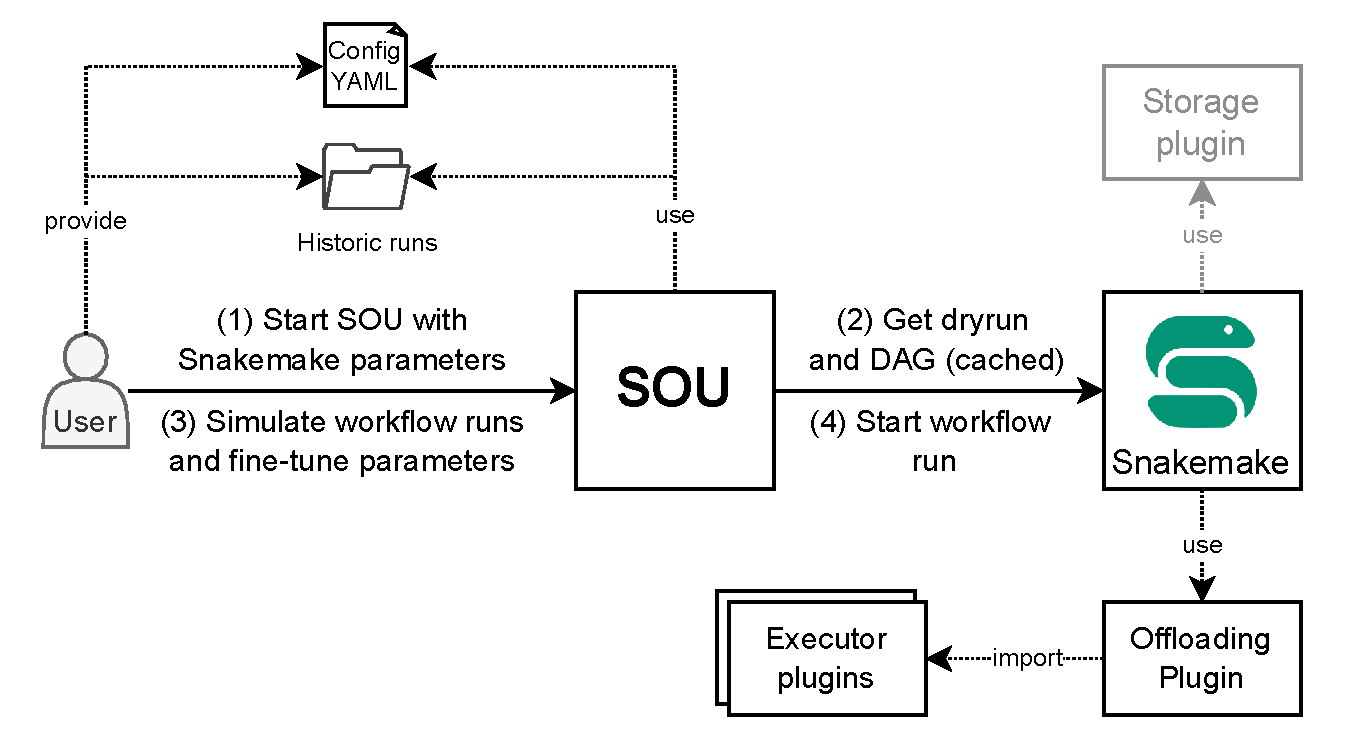
\includegraphics[width=1\linewidth]{./img/components_overview.drawio.pdf}
    \caption{Overview of offloading-related software components}
    \label{fig:components_overview}
\end{figure}
The Kubernetes executor plugin extends an existing Snakemake catalog package to integrate with the Offloading Plugin. 
To analyze the cost of the workflow, we set the cost factor parameters in the SOU configuration file to the values shown in Table~\ref{tab:unit-cost-factors} in Section~\ref{sec:approach}.

\subsubsection{Workflows and Experimental Data}
We evaluate our approach using the real-world bioinformatics workflows rna-seq-star-deseq2, stained-glass and dna-seq-varlociraptor from the Snakemake Workflow Catalog shown in Table~\ref{tab:workflow-comparison}.

These are among the 10 most popular workflows adhering to the catalog standards. They were selected to cover a variety of workflow characteristics, such as the number of tasks and jobs, the task dependency structure and the makespan.

\paragraph{rna-seq-star-deseq2}
The rna-seq-star-deseq2\footnote{\url{https://github.com/snakemake-workflows/rna-seq-star-deseq2}} workflow performs differential gene expression analysis on RNA sequencing data.
As input data, we use FASTQ files from the Genetic European Variation in Health and Disease (GEUVADIS) project \cite{the_geuvadis_consortium_reproducibility_2013, the_geuvadis_consortium_transcriptome_2013}.
The GEUVADIS project investigates the relationship between human genetic variation and gene expression.
In this context, high-depth RNA sequencing data from lymphoblastoid cell lines derived from 465 individuals has been generated.

\paragraph{stained-glass}
The stained-glass\footnote{\url{https://github.com/mrvollger/StainedGlass}} workflow creates identity heatmaps of genomic sequences.
This allows to visualize large-scale repetitive structures in genomes such as tandem repeats \cite{vollger_stainedglass_2022}.
As input data, we use a FASTA file of the human reference genome.
More specifically, we use the T2T-CHM13 v2.0 assembly, which is the first human genome assembly that includes all chromosomes (except Y) and telomeres \cite{nurk_complete_2022}.
In contrast to the other two workflows, where the number of input files is variable and influences the overall number of jobs, the stained-glass workflow depends only on a single FASTA file as input.
The overall number of jobs is determined by a workflow parameter that controls parallelization of the processing steps.
Still, we require multiple different input files for training and test data.
Therefore, we create input files with varying sizes from the T2T-CHM13 v2.0 assembly by extracting subsets of all available chromosomes with the samtools\footnote{\url{https://www.htslib.org}} suite.

\paragraph{dna-seq-varlociraptor}
The dna-seq-varlociraptor\footnote{\url{https://github.com/snakemake-workflows/dna-seq-varlociraptor}} workflow is an analysis pipeline for the detection and statistical evaluation of small variants (changes in  DNA sequence that involve a few nucleotides) and structural variants (changes involving bigger regions) from DNA sequencing data.
As input data, we use FASTQ files generated by Truong and Boeke \cite{truong_resetting_2017}.
The authors performed whole-genome sequencing on Saccharomyces cerevisiae strains which were humanized - that is, the core histones were replaced with their human counterparts.
Note that the task graph is not a DAG, as cycles can occur if jobs associated with the same task are executed at different stages of the workflow.

\subsection{Experimental Results}

We first train SOU’s makespan and cost predictors by running each workflow five times without offloading, using different input sizes to sample diverse task runtimes.

For evaluation, we run each workflow five more times on a separate fixed test dataset. As summarized in Table~\ref{tab:offloading-experiments}, we performed six experiments per workflow with varying offloading strategies and, when applicable, a chosen deadline per workflow. For the stained-glass workflow, we run only four experiments because LJF and SISF produce identical offloading configurations given their DAG structure. 

Table~\ref{tab:prediction-results} constitutes the principal reference for the presentation of our results. It reports a comparison between the observed median makespan, the predicted makespan, and the number of offloaded jobs, together with the associated costs incurred in the secondary environment. %As evaluation metrics, we employ the normalized deadline adherence score, the mean prediction error and costs in \$. 
The predicted error (PE) shown for the makespan and cost is calculated as follows:
\vspace{0.3em}
\[
\text{PE} = \frac{\text{predicted\_value} - \text{median}(\text{observed\_values})}{\text{median}(\text{observed\_values})}
\]

%\subsubsection{Deadline Adherence\label{subsubsec:deadline-adherence}}
\begin{table}[t]
\caption{Number of tasks and jobs per workflow}
\centering
\footnotesize
\setlength{\tabcolsep}{4pt}
\begin{tabular}{l|ccc}
\textbf{Workflow} & \textbf{\# Tasks} & \textbf{\# Jobs} \\
\hline
a) rna-seq-star-deseq2   & 16 & 135  \\
b) stained-glass         & 10 & 44   \\
c) dna-seq-varlociraptor & 40 & 744 
\end{tabular}
\label{tab:workflow-comparison}
\end{table}

% Figure Makespan and Offloading Dependence
\begin{figure*}[t]
  \centering
  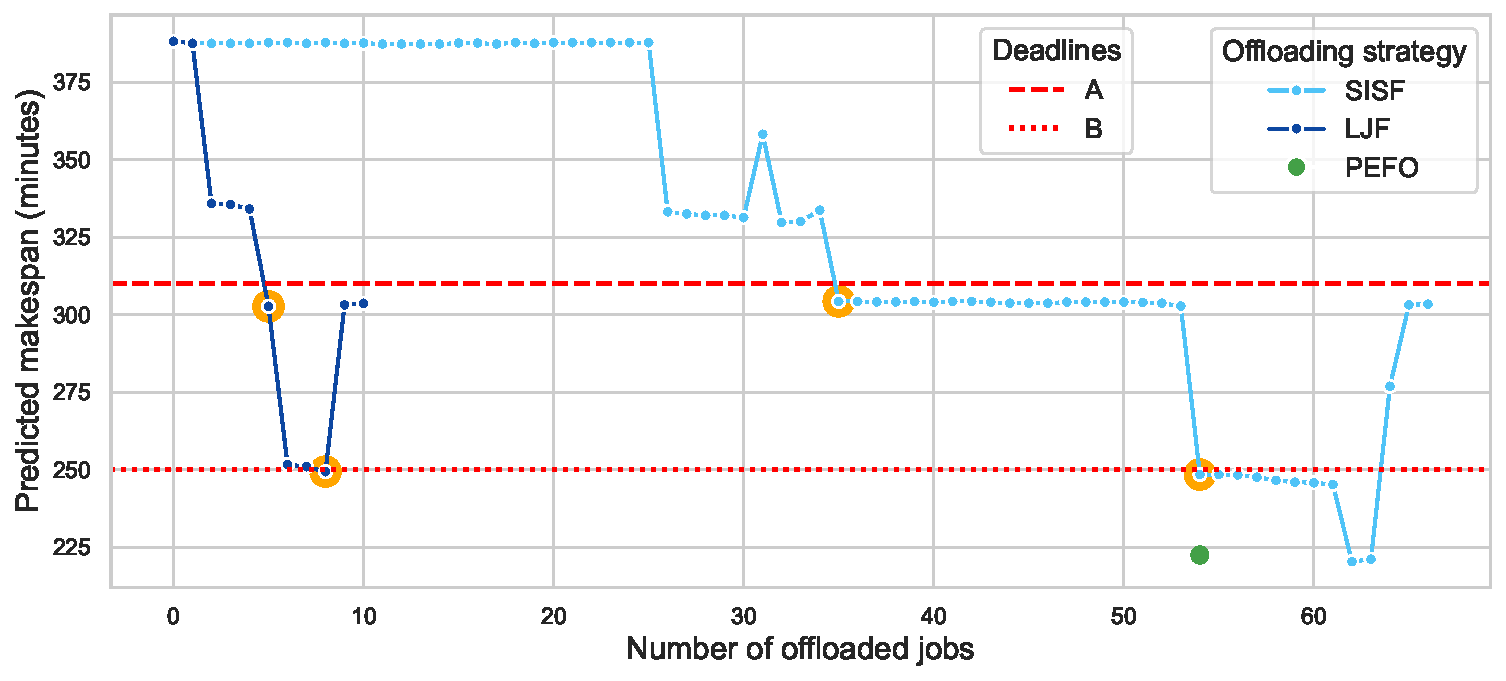
\includegraphics[width=0.8\linewidth]{img/evaluation/workflow_offloading_steps_rna-seq-star-deseq2.pdf}
  \caption{Dependence of workflow makespan prediction on the number of offloaded jobs for rna-seq-star-deseq2}
  \label{fig:makespan-offloading-dependence}
\end{figure*}

% Text on the figure, how it behaves, etc.
Figure~\ref{fig:makespan-offloading-dependence} shows the makespan predictions recorded in each simulation run during the iterative job selection of LJF and SISF (Algorithm~\ref{lst:predict_workflow_makespan}), using the rna-seq-star-deseq2 workflow as an example. The orange points mark the offloading configurations chosen by SOU for the deadlines, corresponding to Table~\ref{tab:prediction-results}. SOU selects the configuration with the fewest offloaded jobs that still meets the deadline. Workflow deadlines were chosen to produce clearly distinct makespan predictions. For comparison, the PEFO makespan prediction is also shown. 

\subsubsection{Dependency between Offloaded Jobs and Makespan Prediction}

\begin{table}[t]
% \small
\caption{Overview of the offloading experiments}
\centering
\begin{tabular}{r|cc}
\textbf{Exp.} & \multicolumn{1}{l}{\textbf{Offl. strategy}} & \multicolumn{1}{l}{\textbf{Deadline}} \\
\hline
1                   & None                                        & N/A                                   \\
2                   & PEFO                                        & N/A                                   \\
3                   & LJF                                         & A                                     \\
4                   & LJF                                         & B                                     \\
5                   & SISF                                        & A                                     \\
6                   & SISF                                        & B                                    
\end{tabular}
\label{tab:offloading-experiments}
\end{table}

In particular, the predicted makespan for SISF remains approximately constant for offloading levels between 0 and 25 jobs. This behavior indicates that, within this range, our heuristic predominantly favors LJF over SISF, because LJF is able to satisfy the deadline constraint after offloading only 6 jobs, in contrast to SISF, which requires the offloading of 35 jobs to meet the same deadline. This behavior is consistent with the objective of minimizing the number of offloaded jobs to still meet the deadline and, consequently, the total execution cost. Therefore, the intuitive expectation that monetary costs increase with a higher number of offloaded jobs while makespan decreases is generally confirmed. This pattern is substantiated by the data in Table~\ref{tab:prediction-results}, which exhibit strong negative Pearson correlation coefficients for makespan and incurring cost ($\rho = -0.925$, $-0.997$, and $-0.845$ for rna-seq-star-deseq2, stained-glass, and dna-seq-varlociraptor, respectively). However, Fig.~\ref{fig:makespan-offloading-dependence} also shows that, for the SISF strategy, the offloading of additional jobs (after 31 and 65 jobs) increases the predicted makespan. In Section~\ref{sec:discussion}, we analyze this behavior and discuss possible reasons for these findings.

\subsubsection{Workflow Makespan Prediction without a Deadline\label{subsubsec:offloading-without-deadline}}
Experiments 1 and 2 compare inactive offloading with offloading guided by the PEFO strategy.
Across all workflows, PEFO reduces median makespans vs inactive offloading by 130~min 28~s (-36.51\%) for rna-seq-star-deseq2, 25~min 16~s (-30.99\%) for stained-glass and 54~min 29~s (-26.07\%) for dna-seq-varlociraptor. Absolute prediction errors range between 1.94\% for rna-seq-star-deseq2 and 12.76\% for dna-seq-varlociraptor. Only rna-seq-star-deseq2 with inactive offloading exceeds the median makespan by 8.63\%.

\subsubsection{Workflow Makespan Prediction with a Deadline \label{subsubsec:offloading-with-deadline}}
To evaluate experiments 3-6 based on Table~\ref{tab:prediction-results}, we compare the LJF and SISF strategies with two different deadlines each.
% General performance
Considering only experiments where the deadline is satisfied by our method, workflows rna-seq-star-deseq2 and stained-glass meet their deadlines with an average slack of approximately 15 minutes. In contrast, dna-seq-varlociraptor consistently violates its deadlines, exceeding them by an average of about 8 minutes.
Deviations in the median makespan from the predicted makespan range from 9 seconds to 35 minutes (PE -0.21\% - 16.88\%).
In particular, the largest prediction errors do not occur between workflows. Instead, they appear only for the SISF strategy in the rna-seq-start-deseq2 workflow (PE 10.66\% \& 16.88\%). 

For rna-seq-star-deseq2, the makespan is generally overestimated. It is slightly underestimated only for LJF under deadline B with a PE of -2.48\%. Prediction errors range from -2.48\% (LJF, B) to 16.88\% (SISF, B). Deadline A is satisfied by both offloading strategies, whereas deadline B is met only by SISF. Although the predicted makespans are similar, SISF produces a substantially lower median makespan than LJF for both deadlines, at the cost of higher prediction errors (10.66\%, 16.88\% vs. -2.48\%, 2.80\%).

For stained-glass workload, the makespan is consistently underestimated with relative errors of -0.21\% (A) and -2.32\% (B), while both deadlines are nevertheless met. 

For dna-seq-varlociraptor, the makespan is systematically underestimated, with prediction errors ranging from \(-7.84\%\) (SISF/B) to \(-4.40\%\) (LJF/A). In none of the experiments are the specified deadlines met, as the actual makespan exceeds the deadline by an average of 10 minutes. The LJF scheduling strategy yields a lower median makespan than SISF for both deadline configurations.

\subsubsection{Offloading Costs}

The resulting offloading costs, summarized in Table~\ref{tab:prediction-results}, reveal that the LJF and SISF strategies, although producing higher makespans, still achieve lower overall costs than the naive offloading baseline (PEFO). This highlights a key trade-off between, on the one hand, minimizing execution time by fully utilizing and saturating local compute resources before offloading, and, on the other hand, deliberately satisfying a given deadline while selecting the cost-optimal configuration.
To illustrate the magnitude of improvement achievable within a single workflow, we consider rna-seq-star-deseq2, which exhibits the largest cost differences between strategies. Under PEFO, this workflow incurs a median cost of \$5.151 with a median makespan of 226.90 minutes, whereas the lowest-cost deadline-aware configuration (LJF with a 310-minute deadline) reduces the median cost to \$2.065 while achieving a comparable median makespan of 294.43 minutes. Similar behavior can be observed for dna-seq-varlociraptor, where costs decrease from \$4.097 under PEFO to \$0.708 with LJF and \$1.449 with SISF. In total, deadline-aware strategies achieve an average cost reduction of 52\% compared to PEFO, corresponding to a geometric mean cost factor of 0.48, calculated by forming per-experiment cost ratios (LJF and SISF relative to PEFO) using median observed costs and aggregating these ratios across all applicable workflows and experiments. These examples show that substantial cost reductions can be achieved within the same workflow, even when allowing for moderate increases in makespan.

\begin{table*}[t]
\caption{Makespan and cost prediction results across workflows}
\centering
\footnotesize
\setlength{\tabcolsep}{4pt}
\begin{tabular}{l|l|rrrrrr}
\textbf{Workflow} & \diagbox{\textbf{Metric}}{\textbf{Experiment}}
& \textbf{1} & \textbf{2} & \textbf{3} & \textbf{4} & \textbf{5} & \textbf{6} \\
\cline{3-8}
 &  & \multicolumn{6}{c}{\textbf{Offloading Strategy}} \\
 &  & None & PEFO & LJF & LJF & SISF & SISF \\
\hline
rna-seq-star-deseq2
 & \# Offloaded jobs          & 0 & 27 & 5 & 8 & 35 & 54 \\
 & Pred. Makespan (min)       & 388.20 & 222.50 & 302.67 & 249.37 & 304.27 & 248.45 \\
 & Median Makespan (min)      & 357.37 & 226.90 & 294.43 & 255.70 & 274.97 & 212.57 \\
 & PE Makespan (\%)           & 8.63 & -1.94 & 2.80 & -2.48 & 10.66 & 16.88 \\
 & Deadline (min)             & N/A & N/A & 310 & 250 & 310 & 250 \\
 & Median Cost (\$)           & 0 & 5.151 & 2.065 & 3.805 & 1.715 & 4.831 \\
\hline
stained-glass
 & \# Offloaded jobs          & 0 & 8 & 2 & 6 & N/A & N/A \\
 & Pred. Makespan (min)       & 78.38 & 53.53 & 72.17 & 59.74 & N/A & N/A \\
 & Median Makespan (min)      & 81.53 & 56.27 & 72.32 & 61.17 & N/A & N/A \\
 & PE Makespan (\%)           & -3.87 & -4.86 & -0.21 & -2.32 & N/A & N/A \\
 & Deadline (min)             & N/A & N/A & 75 & 65 & N/A & N/A \\
 & Median Cost (\$)           & 0 & 0.736 & 0.218 & 0.586 & N/A & N/A \\
\hline
dna-seq-varlociraptor
 & \# Offloaded jobs          & 0 & 279 & 28 & 47 & 232 & 325 \\
 & Pred. Makespan (min)       & 199.46 & 134.80 & 173.72 & 159.34 & 178.73 & 159.90 \\
 & Median Makespan (min)      & 209.00 & 154.52 & 181.72 & 168.98 & 187.42 & 173.52 \\
 & PE Makespan (\%)           & -4.56 & -12.76 & -4.40 & -5.70 & -4.64 & -7.84 \\
 & Deadline (min)             & N/A & N/A & 180 & 160 & 180 & 160 \\
 & Median Cost (\$)           & 0 & 4.097 & 0.708 & 1.941 & 1.449 & 2.654 \\
\end{tabular}
\label{tab:prediction-results}
\end{table*}